\begin{figure}[ht!]
  \centering
  \tikzset{every picture/.style={line width=0.75pt}}
  \resizebox*{0.8\linewidth}{!}{%
    \tikzset{every picture/.style={line width=0.75pt}} %set default line width to 0.75pt
  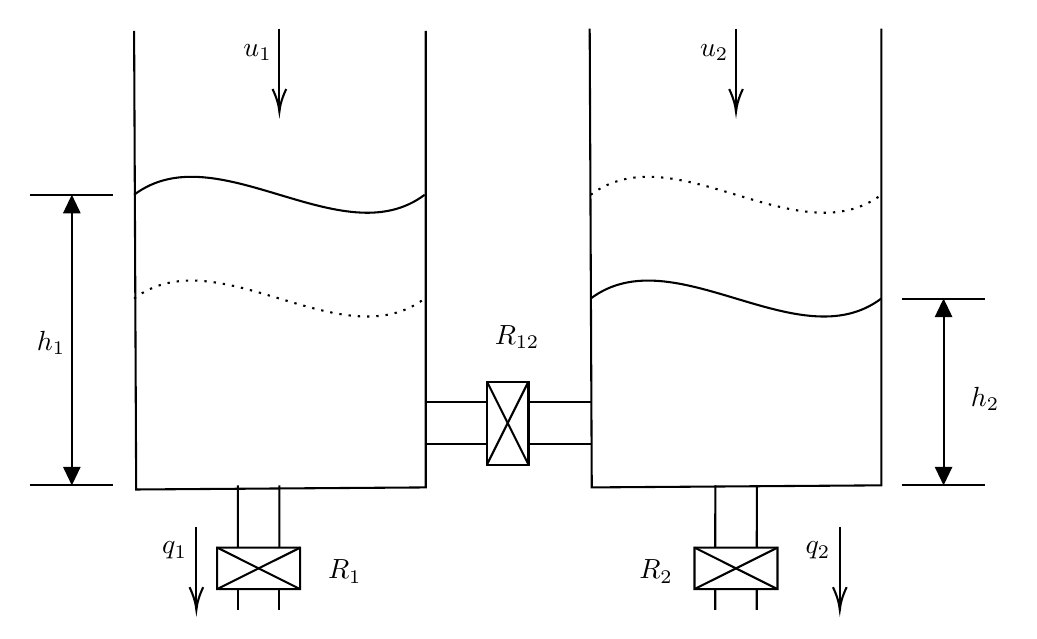
\begin{tikzpicture}[x=0.75pt,y=0.75pt,yscale=-1,xscale=1]
    %uncomment if require: \path (0,459); %set diagram left start at 0, and has height of 459
    %Straight Lines [id:da5688929335924803]
    \draw    (310.5,121) -- (310.5,341) -- (171,342) -- (170,121) ;
    %Straight Lines [id:da5444294116492245]
    \draw    (530,120) -- (530,340) -- (390.5,341) -- (389.5,120) ;
    %Straight Lines [id:da5805131124126722]
    \draw    (200,360) -- (200,398) ;
    \draw [shift={(200,400)}, rotate = 270] [color={rgb, 255:red, 0; green, 0; blue, 0 }  ][line width=0.75]    (10.93,-3.29) .. controls (6.95,-1.4) and (3.31,-0.3) .. (0,0) .. controls (3.31,0.3) and (6.95,1.4) .. (10.93,3.29)   ;
    %Straight Lines [id:da36945578968673487]
    \draw    (510,360) -- (510,398) ;
    \draw [shift={(510,400)}, rotate = 270] [color={rgb, 255:red, 0; green, 0; blue, 0 }  ][line width=0.75]    (10.93,-3.29) .. controls (6.95,-1.4) and (3.31,-0.3) .. (0,0) .. controls (3.31,0.3) and (6.95,1.4) .. (10.93,3.29)   ;
    %Straight Lines [id:da3077937138084411]
    \draw    (310,300) -- (340,300) ;
    %Straight Lines [id:da6773172185122848]
    \draw    (310,320) -- (340,320) ;
    %Shape: Rectangle [id:dp35476624369345366]
    \draw   (340,290) -- (360,290) -- (360,330) -- (340,330) -- cycle ;
    %Straight Lines [id:da9030142425581202]
    \draw    (360,300) -- (390,300) ;
    %Straight Lines [id:da9329287059080266]
    \draw    (360,320) -- (390,320) ;
    %Straight Lines [id:da7833363422326105]
    \draw    (340,290) -- (360,330) ;
    %Straight Lines [id:da26540765973372593]
    \draw    (360,290) -- (340,330) ;
    %Straight Lines [id:da7238601427391023]
    \draw    (470.02,340) -- (470,370) ;
    %Straight Lines [id:da21192498383993508]
    \draw    (450.02,339.99) -- (450,369.99) ;
    %Shape: Rectangle [id:dp4746471043409347]
    \draw   (480,370.01) -- (479.99,390.01) -- (439.99,389.98) -- (440,369.98) -- cycle ;
    %Straight Lines [id:da6336671048955647]
    \draw    (470,389.99) -- (469.98,400) ;
    %Straight Lines [id:da6700066277567417]
    \draw    (450,389.99) -- (449.98,400) ;
    %Straight Lines [id:da928718960478936]
    \draw    (480,370.01) -- (439.99,389.98) ;
    %Straight Lines [id:da1540497075962557]
    \draw    (479.99,390.01) -- (440,369.98) ;
    %Straight Lines [id:da7575667165517417]
    \draw    (240.03,340.01) -- (240.01,370.01) ;
    %Straight Lines [id:da24987185404211631]
    \draw    (220.03,340) -- (220.01,370) ;
    %Shape: Rectangle [id:dp2771887371908066]
    \draw   (250.01,370.02) -- (250,390.02) -- (210,389.99) -- (210.01,369.99) -- cycle ;
    %Straight Lines [id:da9912034440398235]
    \draw    (240,390) -- (240,400) ;
    %Straight Lines [id:da11904000202181764]
    \draw    (220,390) -- (220,400) ;
    %Straight Lines [id:da7480508238760858]
    \draw    (250.01,370.02) -- (210,389.99) ;
    %Straight Lines [id:da7049908339863217]
    \draw    (250,390.02) -- (210.01,369.99) ;
    %Straight Lines [id:da9101133488343268]
    \draw    (240,120) -- (240,158) ;
    \draw [shift={(240,160)}, rotate = 270] [color={rgb, 255:red, 0; green, 0; blue, 0 }  ][line width=0.75]    (10.93,-3.29) .. controls (6.95,-1.4) and (3.31,-0.3) .. (0,0) .. controls (3.31,0.3) and (6.95,1.4) .. (10.93,3.29)   ;
    %Straight Lines [id:da11474588029910615]
    \draw    (460,120) -- (460,158) ;
    \draw [shift={(460,160)}, rotate = 270] [color={rgb, 255:red, 0; green, 0; blue, 0 }  ][line width=0.75]    (10.93,-3.29) .. controls (6.95,-1.4) and (3.31,-0.3) .. (0,0) .. controls (3.31,0.3) and (6.95,1.4) .. (10.93,3.29)   ;
    %Curve Lines [id:da10596831311641142]
    \draw    (170,200) .. controls (210,170) and (270,230) .. (310,200) ;
    %Curve Lines [id:da32042097611565956]
    \draw    (390,250) .. controls (430,220) and (490,280) .. (530,250) ;
    %Curve Lines [id:da9628648357071894]
    \draw  [dash pattern={on 0.84pt off 2.51pt}]  (170,250) .. controls (210,220) and (270,280) .. (310,250) ;
    %Curve Lines [id:da13605436176729158]
    \draw  [dash pattern={on 0.84pt off 2.51pt}]  (390,200) .. controls (430,170) and (490,230) .. (530,200) ;
    %Straight Lines [id:da6375240487876032]
    \draw    (140,202) -- (140,338) ;
    \draw [shift={(140,340)}, rotate = 270] [fill={rgb, 255:red, 0; green, 0; blue, 0 }  ][line width=0.75]  [draw opacity=0] (8.93,-4.29) -- (0,0) -- (8.93,4.29) -- cycle    ;
    \draw [shift={(140,200)}, rotate = 90] [fill={rgb, 255:red, 0; green, 0; blue, 0 }  ][line width=0.75]  [draw opacity=0] (8.93,-4.29) -- (0,0) -- (8.93,4.29) -- cycle    ;
    %Straight Lines [id:da08454244898673535]
    \draw    (120,200) -- (160,200) ;
    %Straight Lines [id:da6622529040678575]
    \draw    (120,340) -- (160,340) ;
    %Straight Lines [id:da8094387172838741]
    \draw    (560,252) -- (560,338) ;
    \draw [shift={(560,340)}, rotate = 270] [fill={rgb, 255:red, 0; green, 0; blue, 0 }  ][line width=0.75]  [draw opacity=0] (8.93,-4.29) -- (0,0) -- (8.93,4.29) -- cycle    ;
    \draw [shift={(560,250)}, rotate = 90] [fill={rgb, 255:red, 0; green, 0; blue, 0 }  ][line width=0.75]  [draw opacity=0] (8.93,-4.29) -- (0,0) -- (8.93,4.29) -- cycle    ;
    %Straight Lines [id:da5524739963534533]
    \draw    (540,250) -- (580,250) ;
    %Straight Lines [id:da7800336719151444]
    \draw    (540,340) -- (580,340) ;
    % Text Node
    \draw (189.5,371.5) node  [align=left] {$\displaystyle q_{1}$};
    % Text Node
    \draw (499.5,371.5) node  [align=left] {$\displaystyle q_{2}$};
    % Text Node
    \draw (354.5,268.5) node  [align=left] {$\displaystyle R_{12}$};
    % Text Node
    \draw (229.5,131.5) node  [align=left] {$\displaystyle u_{1}$};
    % Text Node
    \draw (449.5,131.5) node  [align=left] {$\displaystyle u_{2}$};
    % Text Node
    \draw (130,271.5) node  [align=left] {$\displaystyle h_{1}$};
    % Text Node
    \draw (580,298.5) node  [align=left] {$\displaystyle h_{2}$};
    % Text Node
    \draw (271.5,381.5) node  [align=left] {$\displaystyle R_{1}$};
    % Text Node
    \draw (421.5,381.5) node  [align=left] {$\displaystyle R_{2}$};
  \end{tikzpicture}%
  }
  \caption[System of Coupled Tanks.]{System of Coupled Tanks. Two pumps input
    water into the system, and the water can flow out of the system through each
    tank. The water can also flow from one tank to another, making the state of
    one affect the state of the other. The control objective are the water
    levels of both tanks. The solid and dashed lines representing the water
    levels illustate two configurations, one with \(h_{1}>h_{2}\) and the
    contrary.}%
  \label{fig:tanks-sim}
\end{figure}
